\iffalse
Un'altra caratteristica di PICAT è quella di essere un linguaggio si scripting. In comune ad altri linguaggi di scripting ha infatti un interprete a linea di comando, il fatto di essere dinamicamente tipato. Oltre a ciò prevede numerose funzioni già pronte per essere utilizzate ed è abbastanza espressivo come linguaggio.
\fi

\begin{frame}{Linguaggi di scripting}
	
	\begin{figure}
		\hfill
		
\includegraphics[scale=0.045]{res/terminal}
	\end{figure}

	\begin{itemize}
		\item Interprete a linea di comando
		\item Dinamicamente tipato
		\item Predilezione per flessibilità e brevità
	\end{itemize}
	
	\begin{figure}
		\hspace*{-7cm}
		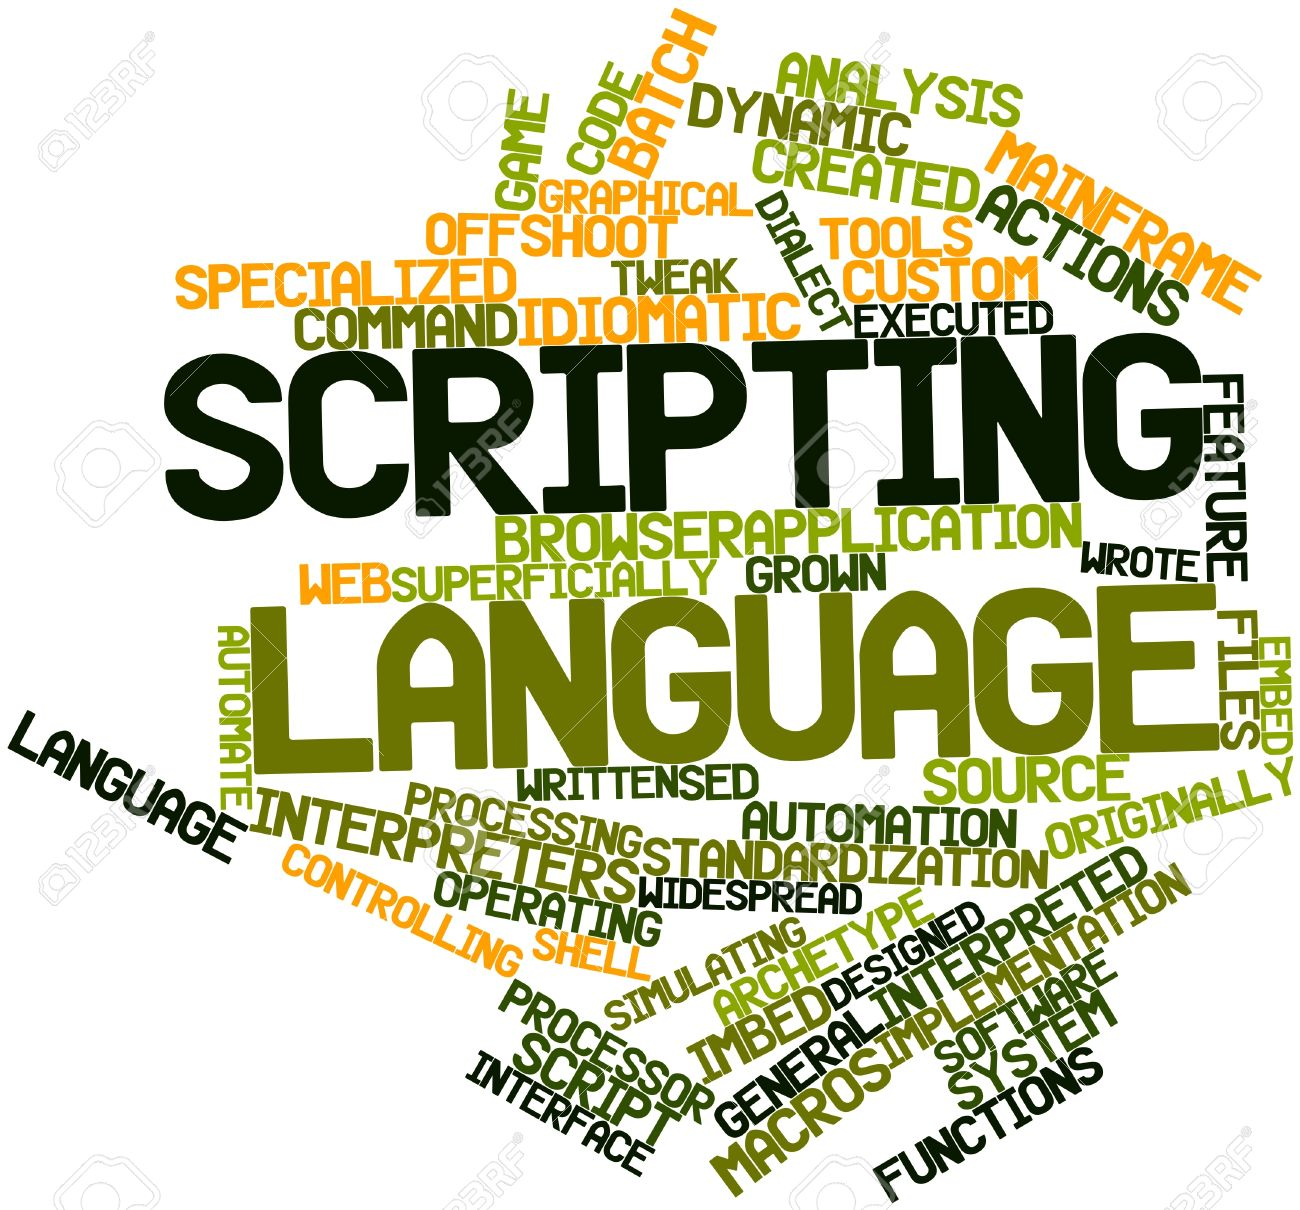
\includegraphics[scale=0.07]{res/scripting}
	\end{figure}

\end{frame}